\section{Реализация решения}\label{chapter3}

В главе \ref{chapter2} было представлено описание решения, которое позволит получить промежуточные состояния потока между вызовами промежуточных операций. Чтобы применить решение на практике реализуем расширение для среды разработки IntelliJ IDEA. 

IntelliJ IDEA -- среда для разработки, основанная на платформе IntelliJ, позволяет разрабатывать программы на нескольких языках программирования, в том числе на java. Функциональность платформы может быть расширена с помощью плагинов, которые могут быть установлены из официального репозитория \cite{jb:plugins}, либо из других источников. Платформа предоставляет разработчикам плагинов API -- классы и интерфейсы, в помощью которых компоненты плагина могут быть интегрированы.
\subsection{Нахождение подходящего вызова}

Для нахождения границ вызова будем использовать API, предоставляемое платформой для работы с исходным кодом. Код представлен в виде $AST$-дерева. Обходя его можно найти цепочки вызовов. Так же интерфейс платформы позволяет определить тип объекта на котором вызывается метод и тип результата. Используя следующие правила, мы сможем классифицировать вызовы внутри цепочки:
\begin{itemize}
	\item Промежуточный - возвращающий объект, реализующий \mintinline{java}{Stream<T>}. .
	\item Завершающий - вызов на наследнике \mintinline{java}{Stream<T>}, возвращающий что-то отличное от \mintinline{java}{Stream<T>}.
\end{itemize}

Учитывая, что положение отладчика может быть отображено на $AST$-дерево, у нас есть возможность обойти его и найти все подходящие цепочки. Кроме того, мы не привязываемся к названиям методов, это упрощает поддержку новых промежуточных операций (вызовы с неподдерживаемым операциями могут отлаживаться: для них будут построены состояния, но переходы восстановить не удастся). Таким образом, можно удовлетворить все требования из \ref{detection}.

\subsection{Построение выражения}
Во второй главе был получен важный результат. Для того, чтобы восстановить все переходы, их нужно восстановить локально для каждого из промежуточных вызовов. При этом информация для восстановления переходов у каждого вызова может различаться. Поэтому будет удобно добавить абстракции, которые позволят каждому вызову модифицировать цепочку, чтобы собрать данные для восстановления перехода. 

Но для всех вызовов верно, что они требуют лишь локальной модификации цепочки: добавления методов до и после. 

Таким образом, достаточно ввести абстракции, которые позволят:
\begin{itemize}
	\item Объявить локальные переменные в выражении для вычисления, нужные для сохранения информации о вычислении.
	\item Добавить промежуточные вызовы в цепочку до и после себя
	\item Преобразовать собранную информацию в процессе запуска выражения к виду, удобному для дальнейшей интерпретации.
\end{itemize}

Очень упрощенно, структура фрагмента кода для вычисления с точки зрения одной операции будет выглядеть следующим образом:

\inputminted{java}{chapter3/code/EvalCode.java}

Пример сгенерированного кода есть в приложении А.

\subsection{Вычисление выражения}
В \ref{code-evaluation} описаны подходы к вычислению произвольного кода внутри отладчика. Так же сделать выбор в пользу загрузки и запуска новых классов. Данная возможность уже присутствует в среде разработки, поэтому не будет подробно останавливаться на том, как этот класс создается. У такого подхода недостаток -- класс загружается как внутренний класс для текущего. При этом сам заменить текущий класс возможности нет. Из-за этого возникает проблема, кто новый класс может обращаться к приватным полям и методам объемлющего класса, но т.к. тот компилировался без него, он новый класс не сможет получить к ним доступ. Для решения этой проблемы используется внутренний класс JDK \mintinline{java}{MagicAccessorImpl} \cite{magic}.

Кроме самого сгенерированного класса, к приватным данные могут пытаться получить доступ и анонимные функции. В текущей версии платформы это приведет к исключению. Но это можно обойти, преобразовав анонимные функции в анонимные классы, которые наследуются от \mintinline{java}{MagicAccessorImpl}. Среда разработки содержит рефакторинги для преобразования анонимных функций в анонимные классы. Мы можем использовать реализацию этих рефакторингов для замены на анонимные классы всех анонимных функций и ссылок на методы.

\subsection{Визуализация}
После завершения вычисления у нас имеется набор промежуточных состояний и переходы между ними. Промежуточные состояния -- это не просто список объектов. Переходы -- это связь между объектам в двух соседних состояниях. наиболее естественно это визуализировать с помощью двух списков объектов и линий-переходов.

При выборе какого-либо значения в списке выделить все объекты, с которыми он связан, затем те с которыми связаны они и т.д. 

И результате был разработан следующий интерфейс:

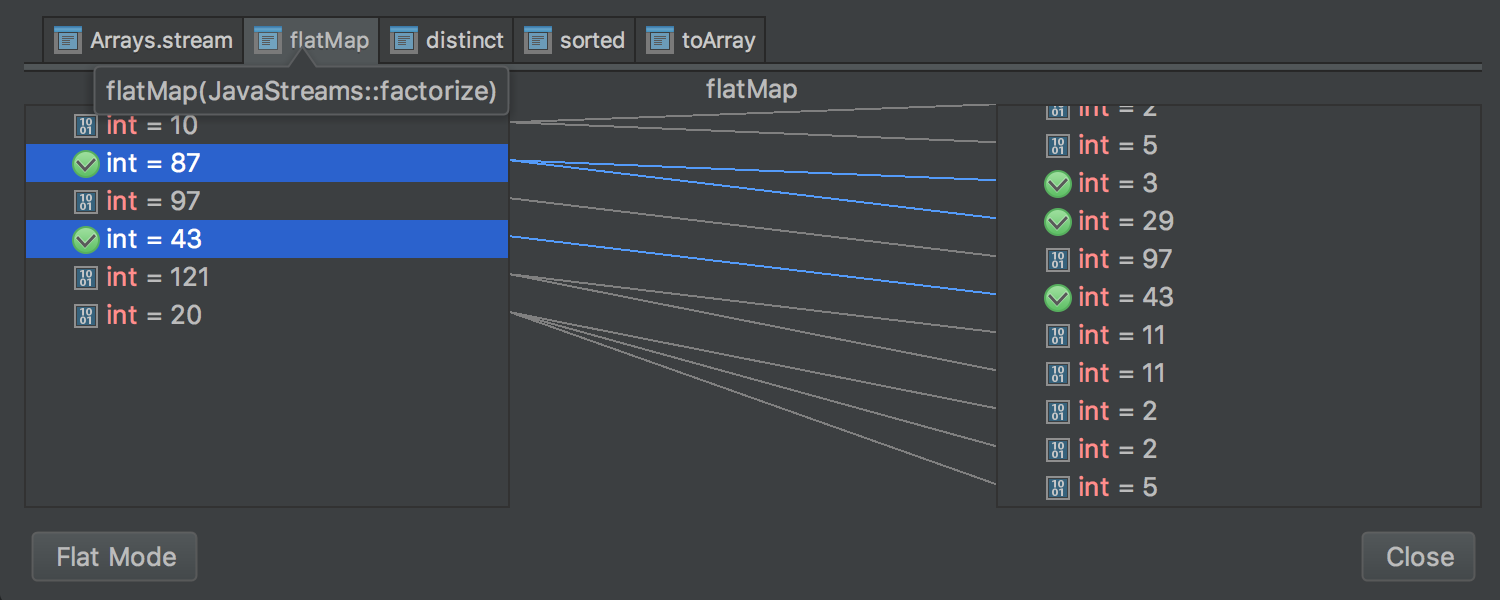
\includegraphics[scale=0.3]{chapter3/img/split-view.png}

Дополнительно, есть возможность просмотреть всю цепочку целиком:

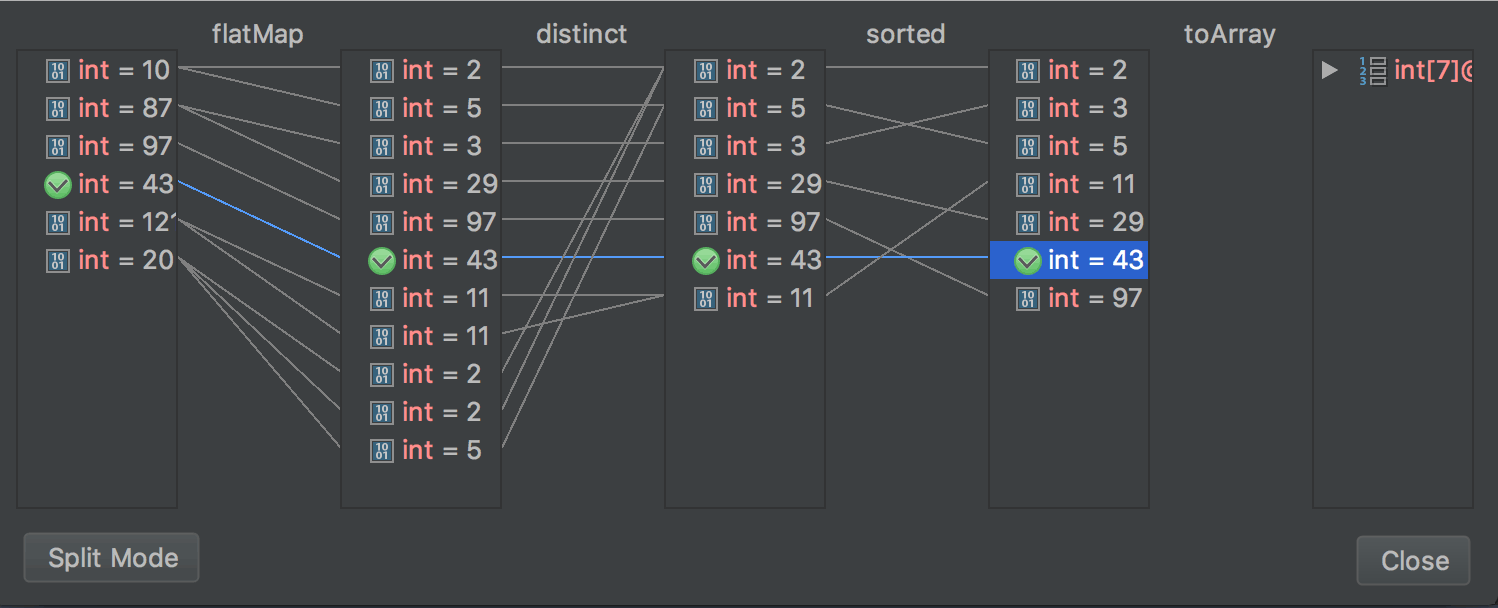
\includegraphics[scale=0.4]{chapter3/img/flat-view.png}










